\subsection{Fehlende Date-Library}

Um Filter für die verschiedenen Zeiträume setzen zu können,
ist es notwendig, ausgehend vom jetzigen Zeitpunkt,
den jeweiligen Start- und Endpunkt eines Zeitraums zu ermitteln.
Wichtig bei der Berechnung von Zeiträumen ist unter anderem auch
die korrekte Einbeziehung der Umstellung von Sommer- und Winterzeit
oder ob eine Woche an einem Sonntag oder Montag beginnt.
Im Web gibt es für solche und ähnliche Berechnungen Bibliotheken
wie beispielsweise \href{https://momentjs.com/docs/}{\textit{Moment.js}}
oder \href{https://date-fns.org/}{\textit{date-fns}}.
Solch eine Bibliothek gibt es allerdings noch nicht im Dart-/Flutterkosmos.
Dementsprechend schrieb ich verschiedene Utility-Funktionen wie
beispielsweise folgende um den letzten Tag eines Monats zu erhalten:
\begin{figure}[H]
    \centering
    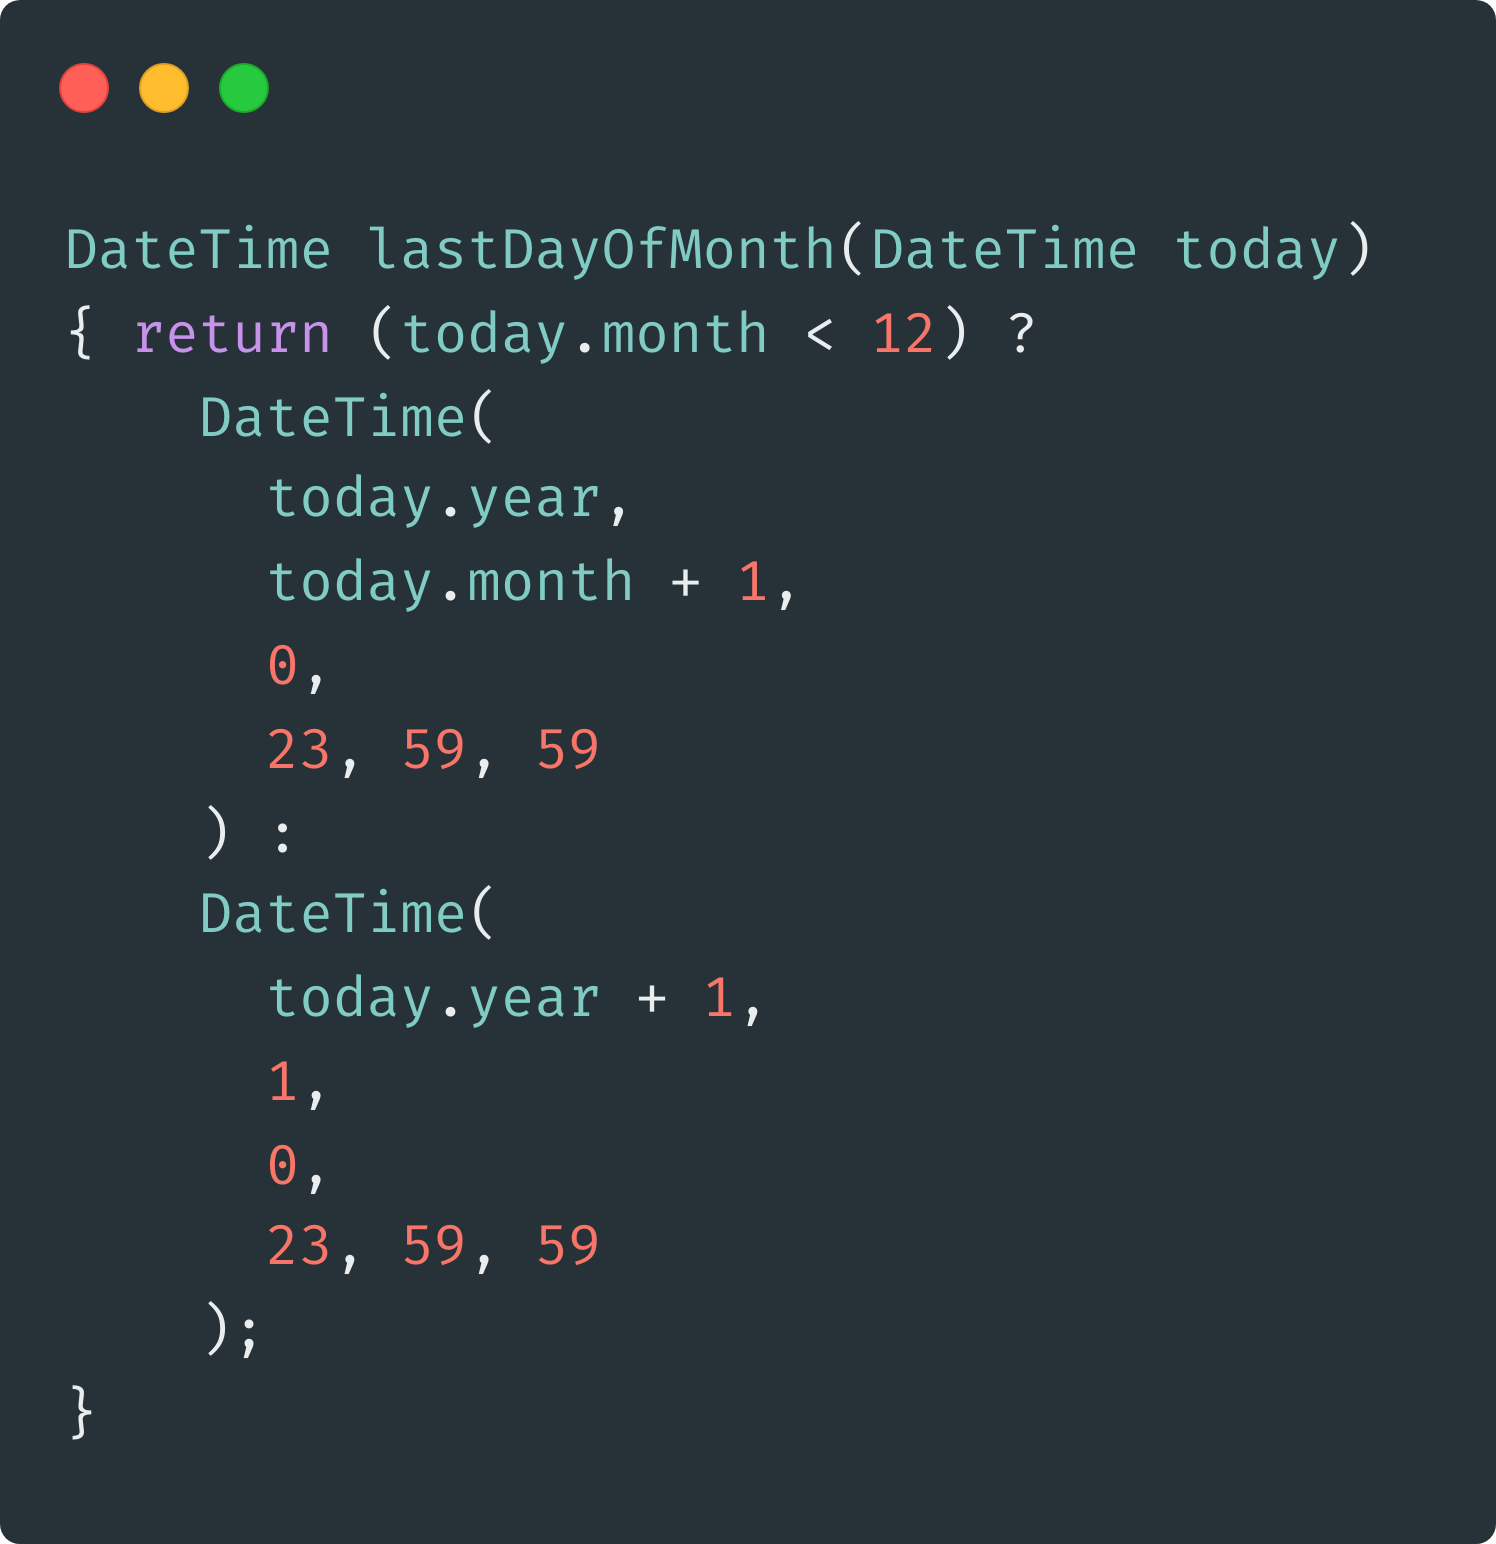
\includegraphics[width=0.4\columnwidth]{last_day_of_month}
    \caption{Dart: Letzter Tag des Monats}
\end{figure}
